%=================================================================
% CSE 4345 — Big Data Analytics
% Week 4, Part 2: Seminal Research & Case Study
% Department of CSE, Premier University
%
% SEMINAL PAPERS:
%   Dean & Ghemawat (2004) — MapReduce: Simplified Data Processing
%   on Large Clusters. OSDI 2004. (cited >21,000 times)
%
%   Chang et al. (2006) — Bigtable: A Distributed Storage System
%   for Structured Data. OSDI 2006. (cited >13,000 times)
%
% CASE STUDY:
%   Facebook Data Infrastructure (2008–2012) — Hive on MapReduce
%   for petabyte-scale analytics + HBase for real-time messaging
%=================================================================

\documentclass[aspectratio=169,10pt]{beamer}

%---------- Packages ----------
\usepackage[utf8]{inputenc}
\usepackage[T1]{fontenc}
\usepackage{booktabs}
\usepackage{xcolor}
\usepackage{tikz}
\usetikzlibrary{shapes.geometric, positioning, arrows.meta, decorations.pathreplacing}
\usepackage{amsmath}
\usepackage{graphicx}
\usepackage{multicol}
\usepackage{enumerate}
\usepackage{array}

%---------- Theme ----------
\usetheme{Madrid}

%---------- Premier University Color Identity ----------
\definecolor{PUNavy}{RGB}{10,36,99}
\definecolor{PUGold}{RGB}{197,151,37}
\definecolor{PULightBlue}{RGB}{210,228,255}
\definecolor{PUTeal}{RGB}{0,100,100}
\definecolor{PUGray}{RGB}{90,90,90}
\definecolor{PURed}{RGB}{160,30,30}
\definecolor{PUGreen}{RGB}{30,120,60}
\definecolor{PUPurple}{RGB}{90,30,120}
\definecolor{PUOrange}{RGB}{190,90,20}

\setbeamercolor{palette primary}{bg=PUNavy, fg=white}
\setbeamercolor{palette secondary}{bg=PUNavy!85, fg=white}
\setbeamercolor{palette tertiary}{bg=PUNavy!70, fg=white}
\setbeamercolor{palette quaternary}{bg=PUNavy, fg=white}
\setbeamercolor{structure}{fg=PUNavy}
\setbeamercolor{title}{bg=PUNavy, fg=PUGold}
\setbeamercolor{subtitle}{fg=white}
\setbeamercolor{frametitle}{bg=PUNavy, fg=PUGold}
\setbeamercolor{alerted text}{fg=PUGold!85!black}
\setbeamercolor{block title}{bg=PUNavy, fg=white}
\setbeamercolor{block body}{bg=PULightBlue!45}
\setbeamercolor{block title alerted}{bg=PUGold!80!black, fg=white}
\setbeamercolor{block body alerted}{bg=PUGold!12}
\setbeamercolor{block title example}{bg=PUTeal, fg=white}
\setbeamercolor{block body example}{bg=PUTeal!10}
\setbeamercolor{section in toc}{fg=PUNavy}
\setbeamercolor{itemize item}{fg=PUGold!80!black}
\setbeamercolor{itemize subitem}{fg=PUNavy!70}

\setbeamertemplate{navigation symbols}{}
\setbeamertemplate{itemize item}{\scriptsize\raise1.5pt\hbox{\textbullet}}
\setbeamertemplate{itemize subitem}{\scriptsize\raise1pt\hbox{--}}

%---------- Section separator ----------
\AtBeginSection[]{
  \begin{frame}[plain]
    \vfill
    \centering
    \begin{beamercolorbox}[sep=12pt,center,shadow=true,rounded=true]{block title}
      \usebeamerfont{title}\insertsectionhead\par
    \end{beamercolorbox}
    \vfill
  \end{frame}
}

%---------- Helper: citation box ----------
\newenvironment{paperbox}[1]{%
  \setbeamercolor{block title}{bg=PUNavy!90,fg=PUGold}
  \setbeamercolor{block body}{bg=PUNavy!6}
  \begin{block}{#1}}{%
  \end{block}}

%---------- Custom footline ----------
\setbeamertemplate{footline}{
  \leavevmode\hbox{%
    \begin{beamercolorbox}[wd=.333\paperwidth,ht=2.25ex,dp=1ex,center]{palette primary}
      \usebeamerfont{author in head/foot}\insertshortauthor
    \end{beamercolorbox}%
    \begin{beamercolorbox}[wd=.334\paperwidth,ht=2.25ex,dp=1ex,center]{palette secondary}
      \usebeamerfont{title in head/foot}\insertshorttitle
    \end{beamercolorbox}%
    \begin{beamercolorbox}[wd=.333\paperwidth,ht=2.25ex,dp=1ex,right]{palette primary}
      \usebeamerfont{date in head/foot}
      \insertframenumber{} / \inserttotalframenumber\hspace*{2ex}
    \end{beamercolorbox}}%
  \vskip0pt%
}

%---------- Title metadata ----------
\title[CSE 4345 \textbar{} Week 4, Part 2]{CSE 4345: Big Data Analytics}
\subtitle{Week 4, Part 2 \textemdash\ Seminal Research \& Case Study}
\author[Dept.\ of CSE]{Department of Computer Science \& Engineering\\[4pt]
       \small Premier University, Chittagong}
\institute{}
\date{Semester 2026}

%=================================================================
\begin{document}
%=================================================================

%----------------------------------------------------------------
% TITLE SLIDE
%----------------------------------------------------------------
\begin{frame}
  \titlepage
\end{frame}

%----------------------------------------------------------------
% PART 2 OVERVIEW
%----------------------------------------------------------------
\begin{frame}{Part 2 Overview — Week 4}
  \begin{columns}[T]
    \column{0.47\textwidth}
      \begin{block}{Today's Agenda}
        \tableofcontents
      \end{block}

    \column{0.50\textwidth}
      \begin{exampleblock}{Seminal Papers Covered}
        \begin{enumerate}
          \item Dean, J., \& Ghemawat, S. (2004).
                \textit{MapReduce: Simplified Data Processing
                on Large Clusters.} OSDI 2004.
          \item Chang, F., et al. (2006).
                \textit{Bigtable: A Distributed Storage System
                for Structured Data.} OSDI 2006.
        \end{enumerate}
      \end{exampleblock}
      \vspace{6pt}
      \begin{alertblock}{Case Study}
        Facebook Data Infrastructure (2008--2012):
        Hive on MapReduce for 30~PB analytics
        + HBase for real-time Messenger at 1~billion messages/day.
      \end{alertblock}
      \vspace{4pt}
      \begin{block}{CLO Addressed}
        \textbf{CLO1} — Understand distributed processing \& storage\\
        \textbf{PLO(a,b)}
      \end{block}
  \end{columns}
\end{frame}

%================================================================
\section{Paper 1 — Dean \& Ghemawat (2004): MapReduce}
%================================================================

%----------------------------------------------------------------
\begin{frame}{Research Landscape: Parallel Processing Timeline}
  \begin{center}
  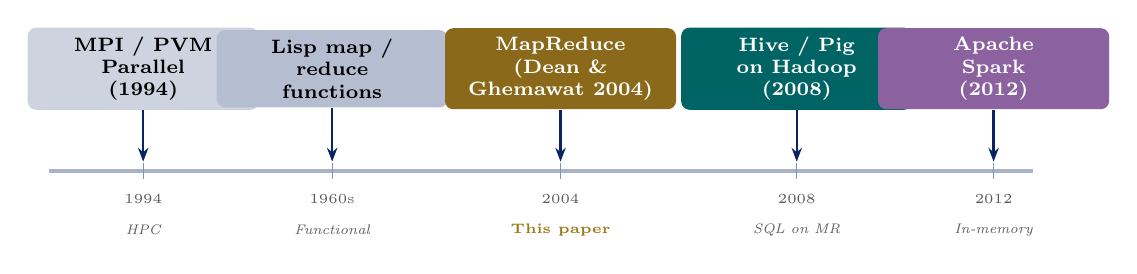
\begin{tikzpicture}[
      nbox/.style={rectangle, rounded corners=3pt, minimum width=2.9cm,
                   minimum height=0.9cm, text width=2.7cm, align=center,
                   font=\scriptsize\bfseries},
      arr/.style={-{Stealth[length=5pt]}, draw=PUNavy, thick}
    ]
    \draw[PUNavy!35, very thick] (0,0) -- (12.5,0);

    \node[nbox, fill=PUNavy!20]              (mpi)  at (1.2, 1.3)
          {MPI / PVM\\Parallel\\(1994)};
    \node[nbox, fill=PUNavy!30]              (lisp) at (3.6, 1.3)
          {Lisp map /\\reduce\\functions};
    \node[nbox, fill=PUGold!70!black, text=white] (mr) at (6.5, 1.3)
          {MapReduce\\(Dean \&\\Ghemawat 2004)};
    \node[nbox, fill=PUTeal, text=white]     (hive) at (9.5, 1.3)
          {Hive / Pig\\on Hadoop\\(2008)};
    \node[nbox, fill=PUPurple!70, text=white](spark)at (12.0,1.3)
          {Apache\\Spark\\(2012)};

    \foreach \x/\y in {1.2/1994, 3.6/1960s, 6.5/2004, 9.5/2008, 12.0/2012}{
      \draw[PUNavy!50] (\x,0.1) -- (\x,-0.1);
      \node[font=\tiny, text=PUGray] at (\x,-0.35) {\y};
    }

    \draw[arr] (mpi)  -- (1.2,  0.12);
    \draw[arr] (lisp) -- (3.6,  0.12);
    \draw[arr] (mr)   -- (6.5,  0.12);
    \draw[arr] (hive) -- (9.5,  0.12);
    \draw[arr] (spark)-- (12.0, 0.12);

    \node[font=\tiny\itshape, text=PUGray]           at (1.2,  -0.75) {HPC};
    \node[font=\tiny\itshape, text=PUGray]           at (3.6,  -0.75) {Functional};
    \node[font=\tiny\bfseries, text=PUGold!80!black] at (6.5,  -0.75) {This paper};
    \node[font=\tiny\itshape, text=PUGray]           at (9.5,  -0.75) {SQL on MR};
    \node[font=\tiny\itshape, text=PUGray]           at (12.0, -0.75) {In-memory};
  \end{tikzpicture}
  \end{center}
  \vspace{3pt}
  \begin{alertblock}{Why MapReduce Was Disruptive}
    MPI required programmers to handle \textbf{process spawning, message passing,
    and failure recovery} manually.
    MapReduce hid all of this behind two functions — \texttt{map} and \texttt{reduce}
    — and handled fault tolerance, data locality, and load balancing \emph{automatically}.
  \end{alertblock}
\end{frame}

%----------------------------------------------------------------
\begin{frame}{Dean \& Ghemawat (2004): Publication Context}
  \begin{columns}[T]
    \column{0.53\textwidth}
      \begin{paperbox}{Full Citation}
        Dean, J., \& Ghemawat, S. (2004).
        \textbf{MapReduce: Simplified Data Processing on Large Clusters.}
        In \textit{Proceedings of the 6th USENIX Symposium on Operating
        Systems Design and Implementation (OSDI '04)},
        pp.~137--150. San Francisco, CA, USA.\\[5pt]
        \textbf{Venue:} USENIX OSDI — Rank A* (CORE)\\
        \textbf{Cited by:} $>$21{,}000 (Google Scholar, 2024)\\
        \textbf{Authors:} Jeffrey Dean \& Sanjay Ghemawat
        (Google Systems Research Group)
      \end{paperbox}
      \vspace{5pt}
      \begin{exampleblock}{The Motivation (from the paper)}
        Google engineers were writing hundreds of special-purpose programs
        to process large datasets.  After noticing that \emph{most programs
        followed the same pattern}, Dean and Ghemawat abstracted it into
        a single framework.  The first internal production use:
        \textbf{building the web search inverted index}.
      \end{exampleblock}

    \column{0.44\textwidth}
      \begin{block}{The Programming Model (1 sentence)}
        \begin{center}
        \large\color{PUNavy}
        \texttt{map(k1,v1)} $\to$ \texttt{list(k2,v2)}\\[8pt]
        \texttt{reduce(k2, list(v2))} $\to$ \texttt{list(v3)}
        \end{center}
      \end{block}
      \vspace{5pt}
      \begin{alertblock}{Classic Example: Word Count}
        \textbf{Map}: for each word $w$ in document, emit $(w, 1)$\\[4pt]
        \textbf{Shuffle}: group all $(w, 1)$ pairs by key $w$\\[4pt]
        \textbf{Reduce}: sum the list of 1s for each $w$\\[4pt]
        $\Rightarrow$ Output: $(w, \text{count})$ for all $w$
      \end{alertblock}
  \end{columns}
\end{frame}

%----------------------------------------------------------------
\begin{frame}{Technical Contribution 1 — Execution Model \& Data Locality}
  \begin{columns}[T]
    \column{0.48\textwidth}
      \begin{block}{MapReduce Execution Flow}
        \begin{enumerate}
          \item \textbf{Split}: input file divided into $M$ splits
                (default 64--128~MB, one split per mapper)
          \item \textbf{Map phase}: $M$ map tasks run in parallel
                on nodes that \emph{hold the input splits}
                (\textbf{data locality} — compute goes to data)
          \item \textbf{Shuffle \& Sort}: map output key-value pairs
                \textbf{partitioned} by key, written to local disk,
                then \textbf{sorted} and transferred to reducers
          \item \textbf{Reduce phase}: $R$ reduce tasks each receive
                all values for a key range; write output to GFS/HDFS
        \end{enumerate}
      \end{block}
      \vspace{4pt}
      \begin{alertblock}{Data Locality Optimisation}
        The master scheduler \textbf{prefers to assign map tasks
        to nodes that already hold the corresponding HDFS block}.
        This avoids network transfer of the (large) input data.
        Only the (smaller) map output crosses the network.
      \end{alertblock}

    \column{0.49\textwidth}
      \begin{center}
      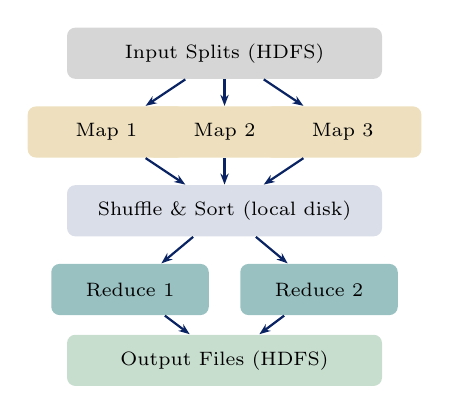
\begin{tikzpicture}[
          ph/.style={rectangle, rounded corners=3pt, minimum width=2.0cm,
                     minimum height=0.65cm, align=center, font=\scriptsize},
          arr/.style={-{Stealth[length=4pt]}, draw=PUNavy, thick}
        ]
        % Input
        \node[ph, fill=PUGray!25, minimum width=4.0cm]
              (inp) at (0, 4.0) {Input Splits (HDFS)};

        % Map tasks
        \node[ph, fill=PUGold!30] (ma) at (-1.5, 3.0) {Map 1};
        \node[ph, fill=PUGold!30] (mb) at (0,    3.0) {Map 2};
        \node[ph, fill=PUGold!30] (mc) at (1.5,  3.0) {Map 3};

        % Intermediate
        \node[ph, fill=PUNavy!15, minimum width=4.0cm]
              (shuf) at (0, 2.0) {Shuffle \& Sort (local disk)};

        % Reduce tasks
        \node[ph, fill=PUTeal!40]  (ra) at (-1.2, 1.0) {Reduce 1};
        \node[ph, fill=PUTeal!40]  (rb) at (1.2,  1.0) {Reduce 2};

        % Output
        \node[ph, fill=PUGreen!25, minimum width=4.0cm]
              (out) at (0, 0.1) {Output Files (HDFS)};

        \draw[arr] (inp)  -- (ma);
        \draw[arr] (inp)  -- (mb);
        \draw[arr] (inp)  -- (mc);
        \draw[arr] (ma)   -- (shuf);
        \draw[arr] (mb)   -- (shuf);
        \draw[arr] (mc)   -- (shuf);
        \draw[arr] (shuf) -- (ra);
        \draw[arr] (shuf) -- (rb);
        \draw[arr] (ra)   -- (out);
        \draw[arr] (rb)   -- (out);
      \end{tikzpicture}
      \end{center}
  \end{columns}
\end{frame}

%----------------------------------------------------------------
\begin{frame}{Technical Contribution 2 — Fault Tolerance \& Stragglers}
  \begin{columns}[T]
    \column{0.52\textwidth}
      \begin{block}{Task-Level Fault Tolerance}
        \begin{itemize}
          \item Master \textbf{pings} each worker periodically;
                worker deemed dead after no response for 5 minutes
          \item All \textbf{completed map tasks} on a dead worker are
                \textbf{re-executed} (output was on local disk, now inaccessible)
          \item Completed \textbf{reduce tasks} are \emph{not} re-executed
                (output is in GFS/HDFS, fault-tolerant already)
          \item A task is \textbf{in-progress} on a dead worker is
                automatically rescheduled on another worker
          \item \textbf{Determinism requirement}: map/reduce functions
                must produce the same output for the same input
                — this makes re-execution semantically correct
        \end{itemize}
      \end{block}
      \vspace{4pt}
      \begin{exampleblock}{Master Fault Tolerance}
        Master writes \textbf{periodic checkpoints} of its data
        structures.  On failure, a new master restores from the
        last checkpoint.  In practice, Google reported that master
        failure was rare and required manual restart.
      \end{exampleblock}

    \column{0.45\textwidth}
      \begin{block}{Straggler Mitigation: Backup Tasks}
        A \textbf{straggler} is a map or reduce task that takes far
        longer than its peers — caused by a slow disk, bad network,
        or noisy CPU.\\[5pt]
        \textbf{Solution}: when a MapReduce job is near completion,
        the master launches \emph{backup copies} of all in-progress tasks.
        Whichever copy finishes first is accepted; the other is killed.\\[5pt]
        \textbf{Result (from the paper)}: backup tasks reduce job
        completion time by up to \textbf{44\%} on a 200-task job with
        one slow machine.
      \end{block}
      \vspace{4pt}
      \begin{alertblock}{Combiner Function}
        Optional \textbf{combiner} runs on the mapper node
        \emph{before} the shuffle — performs partial aggregation.
        In word count: sum local counts before sending to reducers.
        Reduces network transfer by up to \textbf{10$\times$}.
      \end{alertblock}
  \end{columns}
\end{frame}

%----------------------------------------------------------------
\begin{frame}{Impact Today — Dean \& Ghemawat (2004)}
  \begin{columns}[T]
    \column{0.50\textwidth}
      \begin{block}{Direct Descendants \& Legacy}
        \begin{itemize}
          \item \textbf{Hadoop MapReduce} (2006) — open-source Java
                reimplementation; shipped by Yahoo!, Cloudera, Hortonworks
          \item \textbf{Apache Hive} (2009) — SQL-to-MapReduce compiler;
                Facebook's solution for analysts who can't write Java MR
          \item \textbf{Apache Pig} (2008) — dataflow language compiling
                to MapReduce; Yahoo!'s ETL automation tool
          \item \textbf{Apache Spark} (2010) — replaced MapReduce's
                disk-based shuffle with in-memory RDDs;
                Spark's DAG model is a direct response to MR's limitations
          \item \textbf{Google's Dataflow / Flume} (2010+) — Google's
                own successor, which led to Apache Beam (Week 11)
          \item \textbf{AWS EMR, Azure HDInsight} — cloud-managed Hadoop
                MapReduce as a service; still widely used in 2024
        \end{itemize}
      \end{block}

    \column{0.47\textwidth}
      \begin{exampleblock}{CMU 15-721 / Stanford CS246 Perspective}
        \begin{itemize}
          \item CMU 15-721 frames MapReduce as a
                \textbf{shared-nothing query processor}: map = scan +
                project, reduce = aggregate; execution plan is a
                two-stage pipeline with one blocking barrier (shuffle)
          \item Stanford CS246 uses MapReduce for
                \textbf{graph algorithms} (PageRank iteration) and
                \textbf{matrix multiplication} — showing that the
                model extends far beyond word count
          \item Both courses note MapReduce's fundamental limitation:
                multi-pass algorithms require chaining jobs and writing
                intermediate results to HDFS — Spark's primary motivation
        \end{itemize}
      \end{exampleblock}
      \vspace{4pt}
      \begin{alertblock}{CLO1 Connection}
        MapReduce operationalises the \textbf{Velocity} dimension of
        Big Data: processing TBs of logs in hours rather than days.
      \end{alertblock}
  \end{columns}
\end{frame}

%================================================================
\section{Paper 2 — Chang et al.\ (2006): Bigtable}
%================================================================

%----------------------------------------------------------------
\begin{frame}{Chang et al.\ (2006): Publication Context \& Data Model}
  \begin{columns}[T]
    \column{0.53\textwidth}
      \begin{paperbox}{Full Citation}
        Chang, F., Dean, J., Ghemawat, S., Hsieh, W.~C., Wallach, D.~A.,
        Burrows, M., Chandra, T., Fikes, A., \& Gruber, R.~E. (2006).
        \textbf{Bigtable: A Distributed Storage System for Structured Data.}
        In \textit{Proceedings of the 7th USENIX OSDI}, pp.~205--218.
        Seattle, WA, USA.\\[5pt]
        \textbf{Venue:} USENIX OSDI — Rank A*\\
        \textbf{Cited by:} $>$13{,}000 (Google Scholar, 2024)\\
        \textbf{Products using Bigtable:} Google Search,
        Google Maps, Gmail, Google Analytics, YouTube
      \end{paperbox}
      \vspace{5pt}
      \begin{block}{The Data Model (2 lines)}
        \textbf{A Bigtable is a sparse, distributed, persistent
        multi-dimensional sorted map.}\\[4pt]
        Key: (\textbf{row key}, \textbf{column key}, \textbf{timestamp})
        $\;\to\;$ \textbf{byte array value}
      \end{block}

    \column{0.44\textwidth}
      \begin{exampleblock}{Webtable: Storing the Web}
        \scriptsize
        \renewcommand{\arraystretch}{1.2}
        \begin{tabular}{@{}lll@{}}
          \toprule
          \textbf{Row key}     & \textbf{Column}     & \textbf{Value} \\
          \midrule
          \texttt{com.cnn.www} & \texttt{content:}   & \texttt{<html>…} \\
          \texttt{com.cnn.www} & \texttt{anchor:cnnsi}& \texttt{"CNN"} \\
          \texttt{com.cnn.www} & \texttt{anchor:my.look}& \texttt{"CNN.com"} \\
          \texttt{com.bbc.www} & \texttt{content:}   & \texttt{<html>…} \\
          \bottomrule
        \end{tabular}
        \vspace{4pt}
        \begin{itemize}
          \item Row keys in \textbf{reverse-domain order}:
                groups pages from same domain together
          \item Each row access is \textbf{atomic}
          \item Column families (\texttt{content}, \texttt{anchor})
                must be declared; columns within a family are dynamic
          \item Multiple \textbf{timestamped versions} per cell
        \end{itemize}
      \end{exampleblock}
  \end{columns}
\end{frame}

%----------------------------------------------------------------
\begin{frame}{Bigtable Architecture — Tablets, SSTable, Compaction}
  \begin{columns}[T]
    \column{0.50\textwidth}
      \begin{block}{Three-Layer Architecture}
        \begin{itemize}
          \item \textbf{Master}: assigns tablets to tablet servers,
                detects failures, load-balances, manages schema changes.
                Never on the read/write data path.
          \item \textbf{Tablet servers} (100s--1000s): serve reads and
                writes for their assigned tablets (each tablet is a
                contiguous range of rows, 100~MB--200~MB).
          \item \textbf{Chubby} (distributed lock service): Bigtable
                uses Chubby for master election, tablet server
                registration, and schema storage.
                Chubby is built on Paxos consensus.
        \end{itemize}
      \end{block}
      \vspace{5pt}
      \begin{block}{Write Path: Memtable + WAL + SSTable}
        \begin{enumerate}
          \item Write appended to \textbf{commit log} (WAL)
          \item Write inserted into in-memory \textbf{memtable}
                (sorted by key)
          \item When memtable exceeds threshold: frozen, converted
                to an immutable \textbf{SSTable} on GFS
          \item \textbf{Compaction}: periodic merge of SSTables to
                reduce read amplification and reclaim deleted cells
        \end{enumerate}
      \end{block}

    \column{0.47\textwidth}
      \begin{center}
      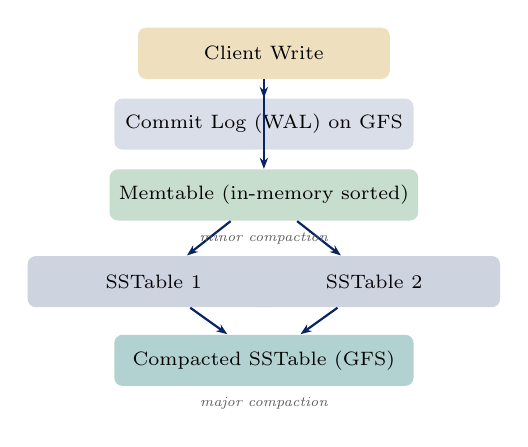
\begin{tikzpicture}[
          bx/.style={rectangle, rounded corners=3pt, minimum width=3.2cm,
                     minimum height=0.65cm, align=center, font=\scriptsize},
          arr/.style={-{Stealth[length=4pt]}, draw=PUNavy, thick}
        ]
        \node[bx, fill=PUGold!30] (cli) at (0, 4.2) {Client Write};

        \node[bx, fill=PUNavy!15, minimum width=3.8cm]
              (wal) at (0, 3.3) {Commit Log (WAL) on GFS};

        \node[bx, fill=PUGreen!25, minimum width=3.8cm]
              (mem) at (0, 2.4) {Memtable (in-memory sorted)};

        \node[bx, fill=PUNavy!20] (ss1) at (-1.4, 1.3) {SSTable 1};
        \node[bx, fill=PUNavy!20] (ss2) at (1.4,  1.3) {SSTable 2};

        \node[bx, fill=PUTeal!30, minimum width=3.8cm]
              (comp) at (0, 0.3) {Compacted SSTable (GFS)};

        \draw[arr] (cli) -- (wal);
        \draw[arr] (cli) -- (mem);
        \draw[arr] (mem) -- (ss1);
        \draw[arr] (mem) -- (ss2);
        \draw[arr] (ss1) -- (comp);
        \draw[arr] (ss2) -- (comp);

        \node[font=\tiny\itshape, text=PUGray] at (0, 1.85)
              {minor compaction};
        \node[font=\tiny\itshape, text=PUGray] at (0,-0.25)
              {major compaction};
      \end{tikzpicture}
      \end{center}
  \end{columns}
\end{frame}

%----------------------------------------------------------------
\begin{frame}{Bigtable vs.\ HBase — Design Correspondence}
  \begin{center}
  \renewcommand{\arraystretch}{1.3}
  \begin{tabular}{@{}lll@{}}
    \toprule
    \textbf{Concept} & \textbf{Bigtable (Google, 2006)} & \textbf{HBase (Apache, 2008)} \\
    \midrule
    Storage layer      & GFS                  & HDFS \\
    Coordination       & Chubby (Paxos)       & ZooKeeper (ZAB protocol) \\
    Tablet unit        & Tablet (100--200~MB) & Region (256~MB default) \\
    Tablet server      & Tablet server        & RegionServer \\
    Master             & Bigtable master      & HBase Master \\
    In-memory store    & Memtable             & MemStore \\
    Sorted file format & SSTable              & HFile (SSTable-compatible) \\
    Compaction         & Minor + Major        & Minor + Major \\
    Bloom filters      & Per SSTable          & Per HFile \\
    Language           & C++                  & Java (JVM) \\
    \bottomrule
  \end{tabular}
  \end{center}
  \vspace{4pt}
  \begin{alertblock}{Key Lesson}
    HBase is to Bigtable exactly what HDFS is to GFS: a faithful
    open-source Java reimplementation.  Understanding Bigtable's
    data model and write path \emph{is} understanding HBase.
  \end{alertblock}
\end{frame}

%================================================================
\section{Case Study — Facebook Data Infrastructure (2008--2012)}
%================================================================

%----------------------------------------------------------------
\begin{frame}{Facebook's Data Scale in 2008}
  \begin{columns}[T]
    \column{0.52\textwidth}
      \begin{block}{The Analytics Challenge}
        By 2008 Facebook had:
        \begin{itemize}
          \item \textbf{100 million active users} producing
                \textbf{15 billion page-views per day}
          \item \textbf{5 TB/day} of event logs (clicks, impressions,
                social graph updates) that needed daily aggregation
                for ad billing and product analytics
          \item A team of analysts and product managers who needed
                \textbf{SQL-like queries} over those logs —
                but could not write Java MapReduce
          \item Oracle data warehouses that could not handle
                \textbf{week-over-week log accumulation}
                (reaching petabyte scale by 2010)
        \end{itemize}
      \end{block}
      \vspace{4pt}
      \begin{exampleblock}{The Decision}
        Facebook deployed Hadoop in 2007, initially for log processing.
        When analysts demanded SQL access, engineers
        \textbf{Joydeep Sen Sarma} and \textbf{Ashish Thusoo}
        built \textbf{Hive} — a SQL-to-MapReduce compiler.
        Hive was open-sourced at VLDB 2009.
      \end{exampleblock}

    \column{0.45\textwidth}
      \begin{center}
      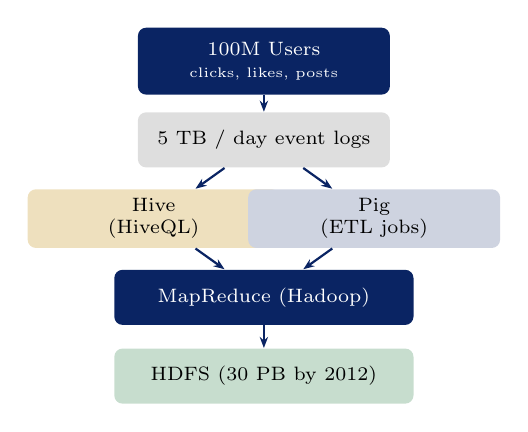
\begin{tikzpicture}[
          fb/.style={rectangle, rounded corners=3pt, minimum width=3.2cm,
                     minimum height=0.7cm, align=center, font=\scriptsize},
          arr/.style={-{Stealth[length=4pt]}, draw=PUNavy, thick}
        ]
        \node[fb, fill=PUNavy, text=white, minimum height=0.85cm]
              (users) at (0, 4.2) {100M Users\\{\tiny clicks, likes, posts}};

        \node[fb, fill=PUGray!20]   (logs) at (0, 3.2) {5 TB / day event logs};

        \node[fb, fill=PUGold!30]   (hive) at (-1.4, 2.2) {Hive\\(HiveQL)};
        \node[fb, fill=PUNavy!20]   (pig)  at (1.4,  2.2) {Pig\\(ETL jobs)};

        \node[fb, fill=PUNavy, text=white, minimum width=3.8cm]
              (mr)   at (0, 1.2) {MapReduce (Hadoop)};

        \node[fb, fill=PUGreen!25, minimum width=3.8cm]
              (hdfs) at (0, 0.2) {HDFS (30 PB by 2012)};

        \draw[arr] (users) -- (logs);
        \draw[arr] (logs)  -- (hive);
        \draw[arr] (logs)  -- (pig);
        \draw[arr] (hive)  -- (mr);
        \draw[arr] (pig)   -- (mr);
        \draw[arr] (mr)    -- (hdfs);
      \end{tikzpicture}
      \end{center}
  \end{columns}
\end{frame}

%----------------------------------------------------------------
\begin{frame}{HBase at Facebook — Real-Time Messenger (2010)}
  \begin{columns}[T]
    \column{0.52\textwidth}
      \begin{block}{The Real-Time Problem}
        While MapReduce served batch analytics, Facebook Messenger
        (launched 2008) required a \textbf{real-time} message store:
        \begin{itemize}
          \item \textbf{1 billion messages/day} at peak
          \item Messages must be \textbf{written and read in $<$100~ms}
                (MapReduce batch latency: hours)
          \item \textbf{High write throughput} (users send bursts);
                \textbf{random point reads} (fetch inbox for a user)
          \item Message threads stored as rows:
                \texttt{row key = user\_id + thread\_id};
                each message as a column with timestamp version
        \end{itemize}
      \end{block}
      \vspace{4pt}
      \begin{alertblock}{HBase: The Right Tool}
        Facebook chose HBase (Bigtable clone) over MySQL sharding
        because:
        \textbf{(1)} automatic tablet splitting handles hotspots;
        \textbf{(2)} memtable absorbs write bursts at microsecond latency;
        \textbf{(3)} column families allow efficient thread-level scans.
      \end{alertblock}

    \column{0.45\textwidth}
      \begin{block}{Scale Numbers (Facebook 2010 HBase deployment)}
        \renewcommand{\arraystretch}{1.25}
        \begin{tabular}{@{}ll@{}}
          \toprule
          \textbf{Metric}         & \textbf{Value} \\
          \midrule
          HBase cluster nodes     & 100            \\
          Messages stored         & $>$135 billion \\
          Peak write rate         & 1M rows / sec  \\
          Median read latency     & $<$10 ms       \\
          Row key space           & user × thread  \\
          Replication factor      & 3 (via HDFS)   \\
          Daily compaction volume & $\sim$1 TB     \\
          \bottomrule
        \end{tabular}
      \end{block}
      \vspace{5pt}
      \begin{exampleblock}{Open-Source Contribution}
        Facebook's Hadoop + Hive + HBase deployment was documented
        in Thusoo et al.\ (VLDB 2009 \& 2010) and drove
        $>$500 patches to Apache Hadoop / HBase between 2008--2012.
      \end{exampleblock}
  \end{columns}
\end{frame}

%----------------------------------------------------------------
\begin{frame}{Lessons Learned \& Discussion Questions}
  \begin{columns}[T]
    \column{0.52\textwidth}
      \begin{block}{Key Lessons from Facebook's Case}
        \begin{enumerate}
          \item \textbf{Right tool for the workload}: MapReduce for
                batch analytics, HBase for random-access real-time reads —
                a single database cannot serve both optimally
          \item \textbf{SQL lowers the barrier}: Hive's HiveQL let
                hundreds of non-Java analysts query petabyte-scale data;
                tool ergonomics matter as much as raw performance
          \item \textbf{Schema flexibility has a cost}: HBase's schemaless
                column families allowed rapid iteration, but required
                careful key design to avoid hotspotting
          \item \textbf{Compaction is a hidden cost}: HBase compaction
                consumed significant I/O; Facebook had to schedule
                major compactions during off-peak hours
          \item \textbf{Open source as a talent strategy}:
                open-sourcing Hive attracted 100+ external contributors
                and made it an industry standard within 3 years
        \end{enumerate}
      \end{block}

    \column{0.45\textwidth}
      \begin{alertblock}{Discussion Questions \textmd{\tiny (CLO1, CLO4)}}
        \begin{enumerate}
          \item MapReduce's shuffle phase requires \textbf{all map tasks
                to complete} before reducers start.
                Explain why this is a \emph{blocking barrier} and
                describe how Apache Spark's \textbf{narrow vs.\ wide
                transformations} eliminate some of these barriers.
                \textit{[CLO1 — Understand]}
          \item Facebook's HBase row key is
                \texttt{user\_id + thread\_id}.
                If all active users are in the range
                \texttt{1000–1999}, identify the hotspot problem
                and propose a \textbf{row key salting strategy}
                to distribute load evenly across RegionServers.
                \textit{[CLO4 — Apply]}
          \item Bigtable uses \textbf{Chubby} (Paxos) while HBase
                uses \textbf{ZooKeeper} (ZAB).
                Compare the two coordination protocols and explain
                which provides stronger consistency guarantees.
                \textit{[CLO1 — Analyse]}
        \end{enumerate}
      \end{alertblock}
  \end{columns}
\end{frame}

%================================================================
\section{Live Exercise}
%================================================================

%----------------------------------------------------------------
\begin{frame}[fragile]{Live Exercise — MapReduce Word Count in Python (mrjob)}
  \begin{columns}[T]
    \column{0.50\textwidth}
      \begin{block}{Task (20 minutes, pairs)}
        Run a MapReduce word count using
        \textbf{mrjob} (Python MapReduce framework)
        locally — no Hadoop cluster required.\\[5pt]
        \textbf{Goal}: count word frequencies in any text file
        and find the top-10 most frequent words.\\[5pt]
        \textbf{Extension 1}: add a \textbf{combiner} method
        and measure whether it reduces intermediate output size.\\[5pt]
        \textbf{Extension 2}: modify to compute
        \textbf{average word length} per first letter
        (\texttt{group-by = first\_letter},
        \texttt{aggregate = mean(len(word))}).
      \end{block}
      \vspace{4pt}
      \begin{exampleblock}{Install}
        \texttt{\scriptsize pip install mrjob}
      \end{exampleblock}

    \column{0.47\textwidth}
      \begin{exampleblock}{mrjob Word Count Skeleton}
        \scriptsize
        \begin{verbatim}
from mrjob.job import MRJob
from mrjob.step import MRStep

class WordCount(MRJob):

    def steps(self):
        return [MRStep(
            mapper=self.mapper,
            combiner=self.combiner,
            reducer=self.reducer)]

    def mapper(self, _, line):
        for word in line.split():
            yield word.lower(), 1

    def combiner(self, word, counts):
        yield word, sum(counts)

    def reducer(self, word, counts):
        yield word, sum(counts)

if __name__ == '__main__':
    WordCount.run()
        \end{verbatim}
      \end{exampleblock}
  \end{columns}
\end{frame}

%================================================================
\section*{References}
%================================================================

%----------------------------------------------------------------
\begin{frame}{References}
  \begin{block}{Seminal Papers}
    \begin{itemize}
      \item Dean, J., \& Ghemawat, S. (2004).
            MapReduce: Simplified data processing on large clusters.
            \textit{Proceedings of the 6th USENIX OSDI}, 137--150.
      \item Chang, F., Dean, J., Ghemawat, S., et al. (2006).
            Bigtable: A distributed storage system for structured data.
            \textit{Proceedings of the 7th USENIX OSDI}, 205--218.
    \end{itemize}
  \end{block}
  \vspace{4pt}
  \begin{block}{Textbooks \textmd{[TW], [SA], [TE]}}
    \begin{itemize}
      \item \textbf{[TW]} White, T. (2015).
            \textit{Hadoop: The Definitive Guide}, 4th ed.
            (Ch.~2 — MapReduce; Ch.~5 -- HBase). O'Reilly.
      \item \textbf{[SA]} Acharya, S., \& Chellappan, S. (2015).
            \textit{Big Data and Analytics}
            (Ch.~4 — MapReduce programming model). Wiley.
      \item \textbf{[TE]} Erl, T., Khattak, W., \& Buhler, P. (2016).
            \textit{Big Data Fundamentals}
            (Ch.~6 — NoSQL and column-family stores). Prentice Hall.
    \end{itemize}
  \end{block}
  \vspace{4pt}
  \begin{block}{Case Study Source}
    \begin{itemize}
      \item Thusoo, A., et al. (2009).
            Hive: A warehousing solution over a map-reduce framework.
            \textit{Proceedings of the VLDB Endowment, 2}(2), 1626--1629.
    \end{itemize}
  \end{block}
\end{frame}

%----------------------------------------------------------------
\begin{frame}{Closing — Week 4, Part 2}
  \begin{columns}[T]
    \column{0.52\textwidth}
      \begin{block}{Key Takeaways}
        \begin{itemize}
          \item MapReduce (2004) proved that \textbf{functional decomposition
                into map + reduce} enables automatic fault tolerance,
                data locality, and parallelism — turning distributed
                programming into a matter of writing two functions
          \item Bigtable (2006) showed that a \textbf{sparse, sorted
                multi-dimensional map} is the right primitive for
                structured data at web scale — HBase is its open-source twin
          \item Facebook's deployment demonstrated that
                \textbf{MapReduce (batch) and Bigtable/HBase (real-time)}
                are complementary, not competing, and most production
                architectures need both
          \item The \textbf{SSTable + memtable + compaction} pattern
                from Bigtable is now the foundation of RocksDB,
                Cassandra, and every modern LSM-tree storage engine
        \end{itemize}
      \end{block}

    \column{0.45\textwidth}
      \begin{alertblock}{Quote of the Week}
        \begin{center}
        \large\itshape
        ``MapReduce is a programming model
        for processing large data sets
        with a parallel, distributed algorithm
        on a cluster.''
        \end{center}
        \begin{flushright}
        \small --- Dean \& Ghemawat (2004)
        \end{flushright}
      \end{alertblock}
      \vspace{6pt}
      \begin{exampleblock}{Part 1 Preview — Week 5}
        \textbf{YARN, File Formats (Parquet / ORC / Avro)}\\[3pt]
        \begin{itemize}\setlength\itemsep{1pt}
          \item YARN resource management model
          \item Columnar formats: Parquet vs.\ ORC
          \item Avro for schema evolution
          \item Format benchmarks: query speedup
        \end{itemize}
      \end{exampleblock}
  \end{columns}
\end{frame}

%=================================================================
\end{document}
%=================================================================
